\section*{Introduction}
\setcounter{figure}{0}
\addcontentsline{toc}{section}{Introduction}  

\subsection*{Project}
\addcontentsline{toc}{subsection}{Project}  

This project was realized as part of our studies in connection with the company "ALL one Robotics". The initial objective was to build a robot to pick apples. Our client had noticed a great shortage of manpower in French and American farms. In France alone, 1 million seasonal workers are needed for the harvest. This labor force remains difficult to find and the crisis of the cider has amplified this phenomenon. Thus, in the United States, only 80\% of the apples would be picked, resulting in significant economic and food losses. This problem has given the idea to our customer to remotely operate the harvest, giving birth to the project "All One Robotics". 

\bigbreak
It is a year-and-a-half project of 12 students of the Ecole Centrale de Lille whose objective is to build a robot capable of picking apples controlled by a user remotely. With the means available and the difficulties encountered, the project turned to the harvest of tomatoes. We had to build a prototype that will facilitate and accelerate the work.

\bigbreak
Our Client, Patrick Kedziora is a French-American entrepreneur and founder of the start-up "All One Robotics". We could also count on coaches from Centrale Lille who helped us throughout the project, especially for the management of such a project: Mr. Denis le Picart and Mr. Roland Marcoin. Finally, we were able to count on the investment of Mr. Kruszewski, a professor at the Ecole Centrale, and his numerous advice throughout the project.

\subsection*{Team members}
\addcontentsline{toc}{subsection}{Team members}  

In this project we were 12 students in the first year of the Ecole Centrale de Lille: Anna Berger, Anna Ducros, Antoine Alessandrini, Aya Skhoun, David Kirov, Héloïse Boyer-Vidal, Maxime Baquet, Noé Luxembourger, Simon Dahy, Simon Kurney, Thomas Jaouën et Victor Guinebertière. 11 of us came from preparatory classes (from all section) and Simon K. was in double degree with his university in Germany. 

\begin{figure}[ht]
    \centering
    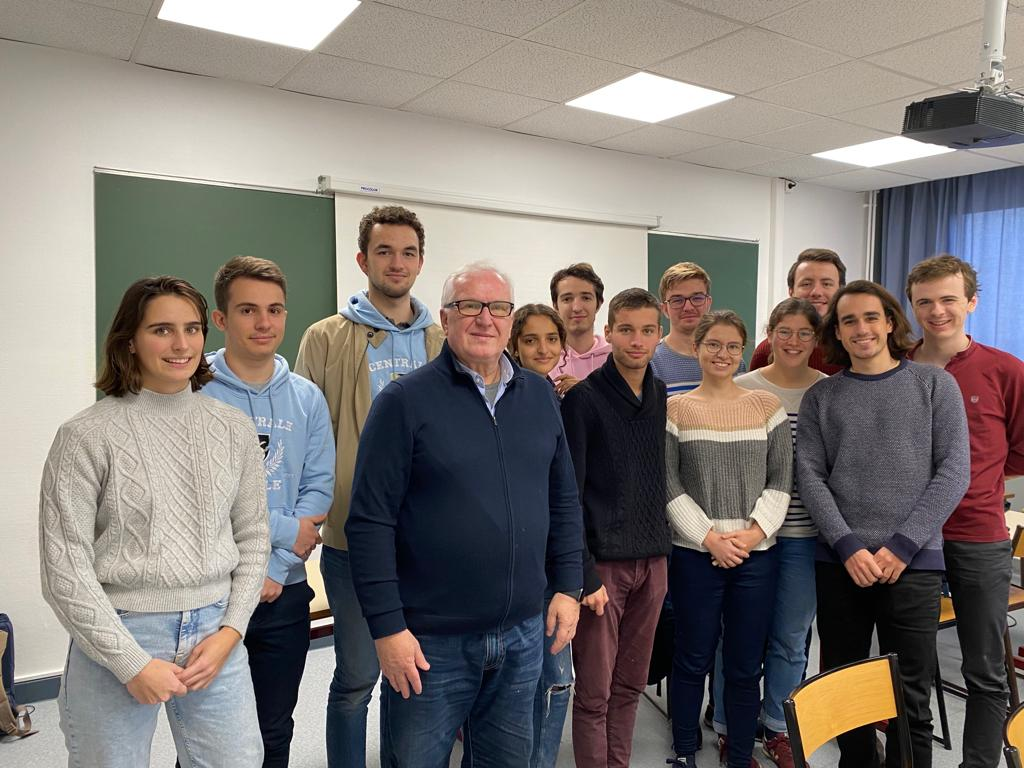
\includegraphics[width=0.8\textwidth]{Images/Members.png}
    \caption{The team with our client}
    \label{fig:Members}
\end{figure}